%\documentclass[handout]{ximera}
\documentclass[nooutcomes]{ximera}

\usepackage{gensymb}
\usepackage{tabularx}
\usepackage{mdframed}
\usepackage{pdfpages}
%\usepackage{chngcntr}

\let\problem\relax
\let\endproblem\relax

\newcommand{\property}[2]{#1#2}




\newtheoremstyle{SlantTheorem}{\topsep}{\fill}%%% space between body and thm
 {\slshape}                      %%% Thm body font
 {}                              %%% Indent amount (empty = no indent)
 {\bfseries\sffamily}            %%% Thm head font
 {}                              %%% Punctuation after thm head
 {3ex}                           %%% Space after thm head
 {\thmname{#1}\thmnumber{ #2}\thmnote{ \bfseries(#3)}} %%% Thm head spec
\theoremstyle{SlantTheorem}
\newtheorem{problem}{Problem}[]

%\counterwithin*{problem}{section}



%%%%%%%%%%%%%%%%%%%%%%%%%%%%Jenny's code%%%%%%%%%%%%%%%%%%%%

%%% Solution environment
%\newenvironment{solution}{
%\ifhandout\setbox0\vbox\bgroup\else
%\begin{trivlist}\item[\hskip \labelsep\small\itshape\bfseries Solution\hspace{2ex}]
%\par\noindent\upshape\small
%\fi}
%{\ifhandout\egroup\else
%\end{trivlist}
%\fi}
%
%
%%% instructorIntro environment
%\ifhandout
%\newenvironment{instructorIntro}[1][false]%
%{%
%\def\givenatend{\boolean{#1}}\ifthenelse{\boolean{#1}}{\begin{trivlist}\item}{\setbox0\vbox\bgroup}{}
%}
%{%
%\ifthenelse{\givenatend}{\end{trivlist}}{\egroup}{}
%}
%\else
%\newenvironment{instructorIntro}[1][false]%
%{%
%  \ifthenelse{\boolean{#1}}{\begin{trivlist}\item[\hskip \labelsep\bfseries Instructor Notes:\hspace{2ex}]}
%{\begin{trivlist}\item[\hskip \labelsep\bfseries Instructor Notes:\hspace{2ex}]}
%{}
%}
%% %% line at the bottom} 
%{\end{trivlist}\par\addvspace{.5ex}\nobreak\noindent\hung} 
%\fi
%
%


\let\instructorNotes\relax
\let\endinstructorNotes\relax
%%% instructorNotes environment
\ifhandout
\newenvironment{instructorNotes}[1][false]%
{%
\def\givenatend{\boolean{#1}}\ifthenelse{\boolean{#1}}{\begin{trivlist}\item}{\setbox0\vbox\bgroup}{}
}
{%
\ifthenelse{\givenatend}{\end{trivlist}}{\egroup}{}
}
\else
\newenvironment{instructorNotes}[1][false]%
{%
  \ifthenelse{\boolean{#1}}{\begin{trivlist}\item[\hskip \labelsep\bfseries {\Large Instructor Notes: \\} \hspace{\textwidth} ]}
{\begin{trivlist}\item[\hskip \labelsep\bfseries {\Large Instructor Notes: \\} \hspace{\textwidth} ]}
{}
}
{\end{trivlist}}
\fi


%% Suggested Timing
\newcommand{\timing}[1]{{\bf Suggested Timing: \hspace{2ex}} #1}




\hypersetup{
    colorlinks=true,       % false: boxed links; true: colored links
    linkcolor=blue,          % color of internal links (change box color with linkbordercolor)
    citecolor=green,        % color of links to bibliography
    filecolor=magenta,      % color of file links
    urlcolor=cyan           % color of external links
}

\title{Bola, Para Bola}
\author{Bart Snapp and Brad Findell}

\outcome{Learning outcome goes here.}

\begin{document}
\begin{abstract}
  We seek to deepen our understanding of parabolas.
\end{abstract}
\maketitle

\begin{teachingnote}
A major purpose here is to explain, from the geometry and also from the algebra, the form of the result:
$y = ax^2 + bx + c$ or $x = ay^2 + by + c$.  
\end{teachingnote}
We've mentioned several times that a parabola is the set of points
that are equidistant from a given point (the focus) and a given line
(the directrix):\index{focus}\index{directrix}
\begin{image}
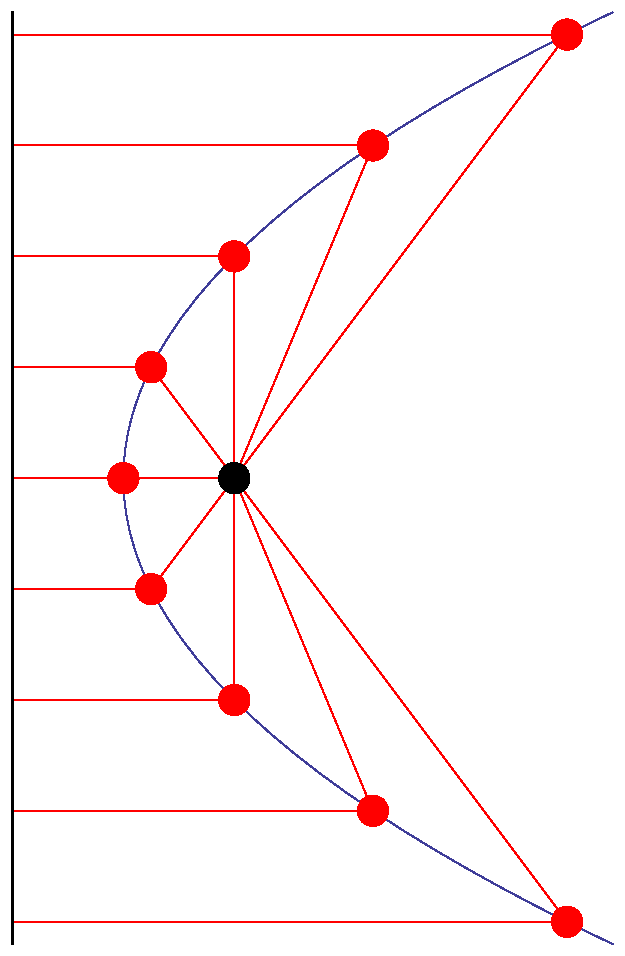
\includegraphics[angle=90,scale=.35]{parabolapointline.pdf}
\end{image}
In this activity we are going to reconcile the definition given
above with the equation that you know and love (admit it!):
\[
y = ax^2 + bx + c
\]

\begin{problem}
How do we compute the distance between two points? Be explicit!
\end{problem}

\begin{problem}
Let's see if we can derive the formula for a parabola with its focus at $(0,1)$ and its directrix being the line $y=0$.
\begin{enumerate}
\item Graph the focus and the directrix, sketch what the parabola might look like, and identify a generic point $(x, y)$.  
\item Draw on the graph the distance from $(x,y)$ to the focus.  Write an expression for this distance.  
\item Draw on the graph the distance from $(x,y)$ to the directrix.  Write an expression for this distance.  
\item Use these two expressions and some algebra to find the formula for the parabola. 
\vspace{.5in}
\item How might you have known, before completing the algebra, that the result would be in the form 
$y = ax^2 + bx + c$? 
\end{enumerate}
\end{problem}
\vspace{.5in}

\begin{problem}
Now derive the formula for a parabola with focus at $(2,1)$ and directrix $y=-1$.
\end{problem}
\vspace{1in}

\begin{problem}
Now derive the formula for a parabola with focus at $(1,-3)$ and directrix $x=3$.  How might you have known, before completing the algebra, the form of the result?   
\end{problem}

\end{document}
